\chapter{Interprocess Communication}

\begin{multicols*}{2}
\section{External Data Representation}

\noindent External Data representation is an agreed standard for representation of data structures and primitive values. Data structure must be flattened before transmission and rebuilt on arrival. \\

\noindent Marshalling converts data items into the form suitable for transmission. Unmarshalling disassembles a message on arrival and restore data items

\subsection{CORBA’s Common Data Representation (CDR)}

\noindent Big / little-endian handling: transmit in sender’s ordering and the recipient translates\\

\noindent Example, flatten a \verb|Person| struct, with \verb|name| (string), \verb|place| (string) and \verb|year| (long) attributes, with value \verb|{"Smith", "London", 1934}|:\\

\begin{center}
\begin{tabular}{ |m{2cm}|c|p{4cm}| } 
    \hline
    Index in sequence of bytes & 4 bytes & Description \\
    \hline 
    0-3   & 5           & length of string \\
    4-7   & \verb|Smit| & \\
    8-11  & \verb|h___| & padded to flush on word boundary \\
    12-15 & 6           & length of string \\
    16-19 & \verb|Lond| & \\
    20-23 & \verb|on__| & padded to flush on word boundary \\
    24-27 & 1934        & \\
    \hline
\end{tabular}
\end{center}

\noindent Assumption: sender and recipient have common knowledge of the order and types of the data items

\subsection{Java Object Serialisation}

\noindent Assumption: the process doing deserialisation has no prior knowledge of the object types in the serialised form\\

\noindent Format: class information, types and names of instance variables, value of instance variables. \\

\noindent Each class is given a handle and no class is written more than once\\

\noindent Example, flatten a \verb|Person| struct, with \verb|name| (string), \verb|place| (string) and \verb|year| (long) attributes, with value \verb|{"Smith", "London", 1934}|:\\

\begin{center}
\begin{tabular}{ |p{1.8cm}|p{1.8cm}|p{1.8cm}|p{1.8cm}| } 
    \hline
    Person & \multicolumn{2}{p{3.6cm}|}{8 bytes version number} & h0 (class handle) \\
    \hline
    3 (number of fields) & int year & string name & string place \\
    \hline
    1934 & 5 Smith & 6 London & h1 (object handle) \\
    \hline
\end{tabular}
\end{center}

\section{Client-Server Communication}

\noindent Validity: the message reaches the destination\\

\noindent Integrity: the message received is identical to the one sent, and no message is delivered more than once

\subsection{Request-Reply Protocol over UDP}

\noindent Message is transmitted without acknowledgements or retires. \\

\noindent UDP is not a reliable communication service:

\begin{itemize}
    \item Integrity: use checksum to detect corrupt packets
    \item Validity: Message validity is not guarantee because it suffers communication omission failures.
\end{itemize}

\noindent To build reliable request-reply protocols over UDP, client uses timeouts when waiting for server’s reply and sends request repeatedly after timeout

\begin{center}
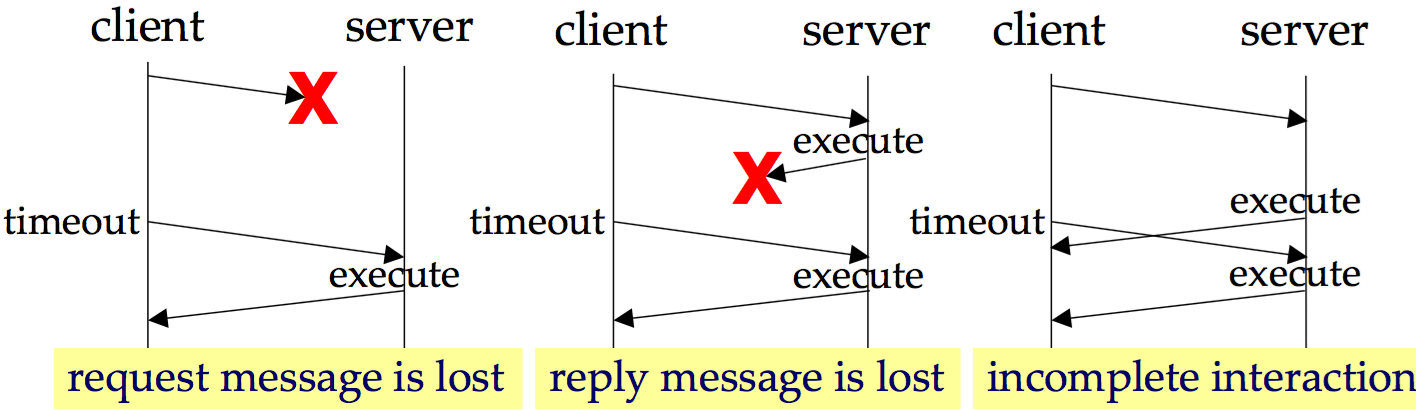
\includegraphics[width=8cm]{udp-interac}
\end{center}

\subsection{Request-Reply Protocol over TCP}

\noindent Message is transmitted with acknowledgement and retries. It is connection-oriented: a connection must be setup before any data are transferred.\\

\noindent TCP is a reliable communication service:

\begin{itemize}
    \item Integrity: use checksums to detect corrupt packets; use sequence numbers to detect duplicate packets
    \item Validity: received packets are acknowledged; use timeouts and retransmission to deal with lost packets.
\end{itemize}

\noindent Reducing Overhead: reuse a single TCP connection to send multiple requests

\subsection{Idempotent and Non-idempotent Operation}

\noindent Idempotent operations: can be performed repeatedly with the same effect as if performed exactly once\\

\noindent Non-idempotent operations: if performed repeatedly have different effects from if performed exactly once


\end{multicols*}
